\section{Hephaestus}\label{sec:hephaestus}

Hephaestus~\cite{rbonifacio:sbcars2009} is a publicly\footnote{http://bit.ly/iRMMZM} available product derivation
tool~\cite{deelstra:2005}, which receives contributions from different
institutions (Federal University of Pernambuco, University of S\~{a}o
Paulo, University of Bras\'{i}lia).  Initially developed as a proof-of-concept tool for managing
variabilities in use case scenarios~\cite{rbonifacio:aosd2009}, Hephaestus
provides a declarative and executable specification in Haskell of  a compositional~\cite{kastner:2008} and parametric approach
for managing variability in use case scenarios.
Currently, Hephaestus supports variability in different types of assets, ranging
from business processes and Simulink models to source code; and
it has been used as the derivation tool in a industrial-strength product line~\cite{ferreira:2010}.

For the initial purpose of the tool, we first implemented:

\begin{itemize}
\item specific data types representing use case model (UCM), feature model (FM), and configuration knowledge (CK) model~\cite{gpbook},
  which relates feature expressions in propositional logic to transformations that
 deal with variability in use cases;

\item specific functions that solve SPL variabilities in use case scenarios, by selecting use cases or scenarios
  from an SPL model, composing them, and binding parameters according to specific
  feature configurations. In addition, Hephaestus
  provides a \texttt{build} function that behaves like an interpreter
  for the configuration knowledge and is responsible for building a
  specific product given a selection of features, i.e., a feature configuration (FC).

\end{itemize}

Figure~\ref{fig:hephaestus-initial-code} presents a piece of code of the
initial implementation of Hephaestus, highlighting data types related to configuration knowledge
(lines \ref{ck-i-1}-\ref{ck-f-1})
and a corresponding interpreter (the \texttt{build} function, in lines \ref{build-i-1}-\ref{build-f-1}) and the signature of
the transformation functions (line \ref{transf-1}). The configuration knowledge relates the problem space (through a feature expression) to the solution space (through a list of asset transformations). Each transformation solves a piece of variability in the SPL asset base. The \texttt{build} function has four input
artifacts (FM, FC, CK, and SPL) and generates a product instance. The \textit{build} process evaluates the rows of the CK, validating each feature expression
according to the FC--- the set of features that characterizes a given product. If a feature expression of the CK is true for
the given FC, then the corresponding transformations are applied to the generated product.
In addition, this code snippet also shows the
initial representation of the \texttt{SPLModel} (lines \ref{splmodel-i-1}-\ref{splmodel-f-1}) and \texttt{InstanceModel}
(lines \ref{instancemodel-i-1}-\ref{instancemodel-f-1})
data types. \texttt{SPLModel} wraps artifacts whose variability management addressed by the tool and their variability as described by the feature model field, whereas \texttt{InstanceModel} wraps assets after a transformation reducing variability has been applied to them. Eventually, all such variability is removed and the \texttt{InstanceModel} value corresponds to the encompassed configuration field. The \texttt{exportProduct} function (lines \ref{exportP-i-1}-\ref{exportP-f-1}) generates a \LaTeX\ representation of a product-specific use case model.

\begin{figure}
%\begin{small}
%\begin{verbatim}
\begin{lstlisting}
type ConfigurationKnowledge = [ConfigurationItem] *'\label{ck-i-1}'*
data ConfigurationItem = ConfigurationItem {
  expression = FeatureExpression,
  transformations = [Transformation]
} *'\label{ck-f-1}'*

build :: FeatureModel *'\label{build-i-1}'*
      -> FeatureConfiguration
      -> ConfigurationKnowledge
      -> SPLModel
      -> InstanceModel
build fm fc ck spl = derive ts spl emptyInstance
where
    ts = concat [transformations c | c <- ck, eval fc (expression c)]
    ucmodel       = splUCM spl
    emptyUCM      = ucmodel { useCases = [] , aspects = [] }
    emptyInstance = InstanceModel fc emptyUCM *'\label{build-f-1}'*

derive [] spl product = product
derive (t:ts) spl product = derive ts spl (t spl product)

type Transformation = SPLModel -> InstanceModel -> InstanceModel *'\label{transf-1}'*

data SPLModel = SPLModel { *'\label{splmodel-i-1}'*
   splFeatureModel :: FeatureModel,
   splUCM :: UseCaseModel
} *'\label{splmodel-f-1}'*

data InstanceModel = InstanceModel { *'\label{instancemodel-i-1}'*
   featureConfiguration :: FeatureConfiguration,
   ucm :: UseCaseModel
} *'\label{instancemodel-f-1}'*

exportProduct :: Path -> InstanceModel -> IO () *'\label{exportP-i-1}'*
exportProduct t product = do
  exportUcmToLatex (t ++ ``/doc.tex'') (ucm product) *'\label{exportP-f-1}'*

exportUcmToLatex = ...
\end{lstlisting}
\caption{Code snippet of the initial implementation of Hephaestus}
\label{fig:hephaestus-initial-code}
%\end{verbatim}
%\end{small}
\end{figure}


% \begin{figure*}
% \begin{center}
% \includegraphics[scale=0.7]{imagens/hephaestus01.eps}
% \end{center}
% \caption{Feature model and code snippet of the initial implementation
%   of Hephaestus. Note that, in this version, all features are mandatory.}
% \label{fig:hephaestus-initial-code}
% \end{figure*}


\subsection{Hephaestus evolution} \label{hp-evolution}


%Hephaestus was extended to use MSVCM in practice. Thus, starting from a prototype for
%experimenting with MSVCM, we evolved Hephaestus into a tool that could be used by students
%and practitioners.  Additionally, within a short period of time, we had to extend
%Hephaestus in another direction, so that it could manage variability not only in use case
%scenarios, but also in higher level requirements and source code
%(by selecting specific files that should be compiled as well by
%starting a preprocessing engine to solve variability in source
%code).

In the context of a R\&D project, Hephaestus was used as a replacement for a proprietary tool that was used to
manage variabilities in an industrial-strength product line~\cite{ferreira:2010},
in which new product assets should be exported as a consequence of the
\texttt{build} process. Hephaestus thus evolved so that it could manage variability not only in use case
scenarios, but also in higher level requirements and source code (by selecting specific files that should be compiled as well as by
starting a preprocessing engine to solve variability in source
code). We show the configuration of both releases in 
%right-hand side of Figure~\ref{fig:hephaestus-fm-02}, while on
%the left-hand side we show the feature model of the first implementation.
Figures~\ref{fig:hephaestus-conf1a} and~\ref{fig:hephaestus-conf1b}.

%\begin{figure*}[bth]
%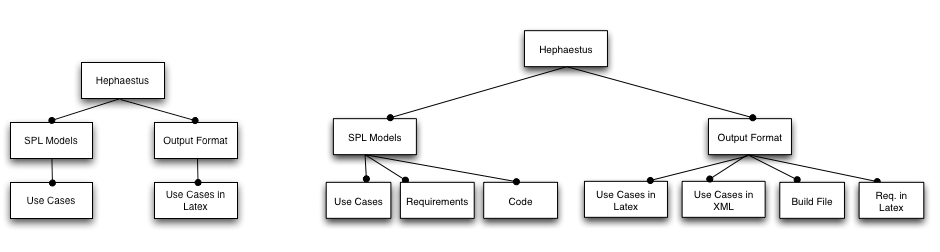
\includegraphics[scale=0.6]{imagens/confs.png}
%\caption{Configurations of Hephaestus in the first two releases.}
%\label{fig:hephaestus-fm-02}
%\end{figure*}


\begin{figure*}[bth]
\begin{center}
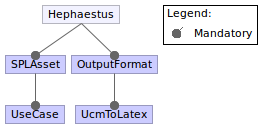
\includegraphics[scale=0.6]{imagens/conf1a-hp.png}
\caption{Configuration of Hephaestus in the first release.}
\label{fig:hephaestus-conf1a}
\end{center}
\end{figure*}


\begin{figure*}[bth]
\begin{center}
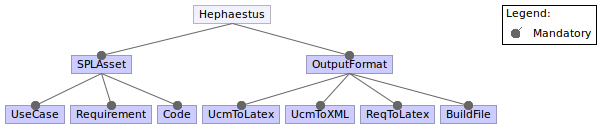
\includegraphics[scale=0.6]{imagens/conf1b-hp.png}
\caption{Configuration of Hephaestus in the second release.}
\label{fig:hephaestus-conf1b}
\end{center}
\end{figure*}



% \begin{figure*}[bth]

% \subfigure[Feature model of the Hephaestus first release]{
% \includegraphics[scale=0.65]{imagens/fm-hephaestus01.eps}
% \label{fig:fm01}
% }
% \subfigure[Feature model of the Hephaestus version tailored to the
% TaRGeT product line]{\includegraphics[scale=0.5]{imagens/fm-hephaestus02.eps}
% \label{fig:fm02}
% }
% \caption{Feature model of the first two releases.}
% \label{fig:hephaestus-fm-02}
% \end{figure*}

In order to achieve these goals, new data types and transformations were required, as
well as part of the existing code had to change. Precisely, to introduce support for variabilities in 
high-level requirements (or requirements for short) and source code, we had to:

\begin{enumerate}[(a)]
 \item implement new data types for representing requirements and
   references to source code assets.

 \item implement new parsing and output functions for reading/writing requirements and source code assets into/from \hp.

 \item implement new transformations for resolving variabilities in  requirements and source code.
  % Existing transformations vary    according to their complexity, each one requiring 10 to 100 lines of Haskell code.

 \item evolve the configuration knowledge XML parser, so that it could recognize the concrete syntax of the new transformations.

 \item evolve the base product instance used by the \texttt{build} function.

 \item evolve both \texttt{SPLModel} and \texttt{InstanceModel} data types, to wrap new assets.




\end{enumerate}

The evolution of data types and functions of Hephaestus as described previously are shown in 
Figures~\ref{fig:spl-model-with-req-and-code} and~\ref{fig:xml-transformation-parser}. To introduce support for new types of assets, we
have to change both \texttt{SPLModel} (lines \ref{splmodel-i-2}-\ref{splmodel-f-2} in Figure~\ref{fig:spl-model-with-req-and-code}) and \texttt{InstanceModel}
(lines \ref{instancemodel-i-2}-\ref{instancemodel-f-2})
data types, the empty product definition (lines \ref{emptyInstance-i-2}-\ref{emptyInstance-f-2}),
the \texttt{exportProduct} function  (lines \ref{exportP-i-2}-\ref{exportP-f-2}) and 
the \texttt{xml2Transformation} function of the configuration knowledge XML parser (Figure~\ref{fig:xml-transformation-parser})---even though the \texttt{ConfigurationKnowledge} and \texttt{FeatureModel} data types and 
interpreter (\texttt{build} function) present some degree of stability
(we do not have to change their implementation when we introduce variability support for
new assets). Here we could say that the \texttt{SPLModel} and
\texttt{InstanceModel} data types are not open, since to introduce new SPL assets
we have to change the data type definitions. Therefore, current Hephaestus' architecture and implementation is not sufficiently flexible, as we are not able to
introduce new data types (representing the abstract syntax of a new SPL asset) and transformations modularly, thus incurring in a costly extension effort.


%@Ralf: in the phrases above, please feel free to argue that standard Haskell and FP techniques do not address
%       the issue (we are gradually starting to make the case for meta-programming)

In particular, evolving Hephaestus to support source code variability (Figure~\ref{fig:spl-model-with-req-and-code}) required
a new kind of asset into the \texttt{SPLModel}
(\texttt{splComponents}, line \ref{splComponents-2}). This asset is a list of pairs that relate a name to the
relative path of a source code file. The same kind of asset was also
introduced into the \texttt{InstanceModel} (line  \ref{components-2}). Besides that, two other fields were required in the InstanceModel:
(a) \texttt{buildEntries} (line  \ref{buildEntries-2}), which declares pre-processing directives, and
(b) \texttt{preProcessFiles} (line \ref{preProcessFiles-2}), which declares a list of files that should
be pre-processed by a third part tool. These fields are instantiated
when Hephaestus builds a product, considering
the proper transformations of a product configuration.

\begin{figure}
%\begin{small}
%\begin{verbatim}
\begin{lstlisting}
data SPLModel = SPLModel { *'\label{splmodel-i-2}'*
   splFeatureModel :: FeatureModel,
   splUCM :: UseCaseModel,
   splReq :: RequirementModel,
   splComponents :: ComponentModel *'\label{splComponents-2}'*
} *'\label{splmodel-f-2}'*

data InstanceModel = InstanceModel { *'\label{instancemodel-i-2}'*
   featureConfiguration :: FeatureConfiguration,
   ucm :: UseCaseModel,
   req :: RequirementModel,
   components :: ComponentModel, *'\label{components-2}'*
   buildEntries :: [PreprocessingDirective], *'\label{buildEntries-2}'*
   preProcessFiles :: [PreprocessingFiles] *'\label{preProcessFiles-2}'*
} *'\label{instancemodel-f-2}'*

build :: FeatureModel -> FeatureConfiguration 
      -> ConfigurationKnowledge -> SPLModel -> InstanceModel
build fm fc ck spl = derive ts spl emptyInstance
where
    ts = concat [transformations c | c <- ck, eval fc (expression c)]
    ucmodel       = splUCM spl
    emptyUCM      = ucmodel { useCases = [] , aspects = [] }  *'\label{emptyInstance-i-2}'*
    emptyReq      = RM { reqs = [] }
    emptyInstance = InstanceModel fc emptyUCM emptyReq [] [] [] *'\label{emptyInstance-f-2}'*

exportProduct :: FilePath -> FilePath -> InstanceModel -> IO ()  *'\label{exportP-i-2}'*
exportProduct s o product = do
  exportUcmToLatex (o ++ ``/doc.tex'') (ucm product)
  exportRequirementsToLatex (o ++ ``/doc.lst'') (req product)
  exportSourceCode s o product  *'\label{exportP-f-2}'*

exportSourceCode :: FilePath -> FilePath -> InstanceModel -> IO ()
exportSourceCode s o p = do
  copySourceFiles s o (components p)
  exportBuildFile  (o ++ ``/build.lst'') (buildEntries p)
  preprocessFiles (o ++ ``/build.lst'') (preProcessFiles p) o

\end{lstlisting}
\caption{\texttt{SPLModel} and \texttt{InstanceModel} data types, \texttt{emptyInstance} definition and \texttt{exportProduct} function
  after introducing support for managing variabilities in requirements and source code}
\label{fig:spl-model-with-req-and-code}
%\end{verbatim}
%\end{small}
\end{figure}

The piece of code in Figure~\ref{fig:xml-transformation-parser} shows the impact on the \texttt{xml2Transformation} function of the configuration knowledge XML parser. The first version of Hephaestus declares just the
first four case statements on the \texttt{xml2Transformation}
function (lines  \ref{transformations-ucm-i-2}-\ref{transformations-ucm-f-2}). The
\texttt{selectRequirements} transformation (line \ref{transformations-req-2}) deals with variability in the requirements models,
whereas the remaining transformations (lines \ref{transformations-code-i-2}-\ref{transformations-code-f-2}) solve
variability in source code. We could say that the \texttt{exportProduct}
and \texttt{xml2Transformation} functions are not open, since new output formats and
new types of transformations could not be introduced in a modular way. Similar to the lack of open data types, this shortcoming reinforces the insufficient flexibility of Hephaestus' architecture and implementation.

Finally, current Hephaestus' architecture and implementation also has limited configurability: to obtain a new version of Hephaestus managing variability in only a proper subset of the artifacts currently supported (use case, requirements, code), e.g., a version supporting only code and use cases, the change impact is similar to what has been described previously when adding new assets.

\begin{figure}
%\begin{small}
%\begin{verbatim}
\begin{lstlisting}
xml2Transformation :: XmlTransformation -> Parser Transformation
xml2Transformation transformation =
let
  args = ...
  tnsName = xmlTransformationName transformation
in
  case tnsName of
  ``selectScenarios'' -> Success (selectScenarios args) *'\label{transformations-ucm-i-2}'*
  ``selectUseCases'' -> Success (selectUseCases args)
  ``evaluateAspects'' -> Success (evaluateAspects args)
  ``bindParameter'' -> ...  *'\label{transformations-ucm-f-2}'*
  ``selectRequirements'' -> ... *'\label{transformations-req-2}'*
  ``selectComponents'' -> ... *'\label{transformations-code-i-2}'*
  ``selectAndMoveComponent'' -> ...
  ``createBuildEntries'' -> ...
  ``preprocessFiles'' -> ... *'\label{transformations-code-f-2}'*
  otherwise -> Fail ``...''
\end{lstlisting}
\caption{Piece of code used during the configuration knowledge XML parser}
\label{fig:xml-transformation-parser}
%\end{verbatim}
%\end{small}
\end{figure}
